\chapter{The Greeks for Barrier Options}
\label{sec:greeks}

The Greeks are key sensitivities in option pricing that measure how the price of an option changes with respect to various factors such as the underlying asset price, time to maturity, volatility, and interest rates. For barrier options, the calculation of the Greeks is more complex due to the added condition of a barrier, which affects the option's price path and behavior.

For the plots in this section, the parameters are \( S_0 = 40 \), \( K = 50 \), \( T = 1.0 \), \( r = 0.1 \), \( \sigma = 0.2 \), and \( B = 60 \), representing the spot stock price, strike price, time to maturity (in years), risk-free rate, volatility, and barrier level, respectively.




\section{Delta (\(\Delta\))}

Delta for a barrier option measures the sensitivity of the option price to changes in the underlying asset price (\(S\)). It represents the rate of change of the option's price with respect to small changes in the underlying price.
\[
\Delta = \frac{\partial \text{Option Price}}{\partial S}
\]

For \textbf{knock-in} barrier options, delta behaves similarly to that of a standard European option but is influenced by the presence of the barrier. It reflects how changes in the underlying price affect the probability of the barrier being breached and the option becoming active.

Figure~\ref{fig:delta_upout} shows the delta behavior of an up-and-out put option as a function of the underlying stock price (\(S\)). When the stock price is well below the barrier level (\(B\)), delta behaves similarly to a vanilla European put option. As the price approaches the barrier, delta tends toward zero because the likelihood of the option being knocked out increases, reducing its sensitivity.

To further analyze the delta across different barrier options, refer to the table below:
\begin{center}
	\begin{table}[H]
		\begin{tabular}{ | m{3cm} | m{5cm}| m{4cm} | m{4cm}|} 
			\hline
			\textbf{Barrier Type} & \textbf{Price Far from Barrier} & \textbf{Price Near the Barrier} & \textbf{Intuition}  \\
			\hline
			\textbf{Knock-Out} & Similar to vanilla options     & $\Delta \to 0$ as $S \to B$  & Probability of knock-out increases as $S$ nears $B$. \\ 
			\hline
			\textbf{Knock-In}  & $\Delta \approx 0$ far from barrier   & $\Delta \uparrow$ as $S \to B$  & Option becomes active as the price hits the barrier. \\ 
			\hline
		\end{tabular}
		\caption{Delta behavior for different types of barrier options.}
		\label{tab:delta_barrier_options}
	\end{table}
\end{center}
\textbf{Key Intuition:}
\begin{itemize}
	\item \textbf{Knock-Out Options:} Lose their sensitivity as $\Delta$ tends toward $0$ as the likelihood of being knocked out near the barrier increases.
	\item \textbf{Knock-In Options:} Show increasing sensitivity as the underlying price nears the barrier because the probability of activation rises.
\end{itemize}

The visual analysis in Figure~\ref{fig:delta_upout} shows delta behavior for an up and out put option. The insights from the plot matches the intuition from Table~\ref{tab:delta_barrier_options} which provides a comprehensive understanding of how delta behaves across different types of barrier options. Before the stock price hits the barrier, the delta is similar to one of a vanilla option. As the stock price hits the barrier, there is a steep decline in delta as the option is knocked out and the option price is zero.
\begin{figure}[H]
    \centering
    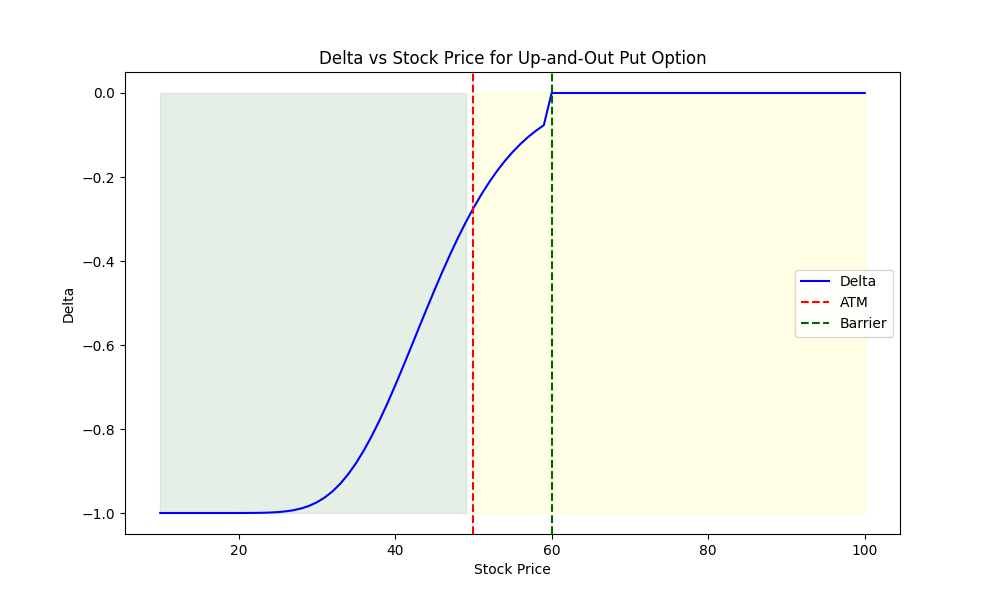
\includegraphics[width=.65\linewidth]{content/images/delta.png}
    \caption{Delta of up-and-out Put Option vs. the Stock Price.}
    \label{fig:delta_upout}
\end{figure}

\subsection{Delta Hedging}

In this section, we retrieve NVDA prices from October 21--25, 2024, using the parameters \( K = 143 \), \( T = 1 \), \( r = 0.046 \), \( \sigma = 0.5 \), and \( B = 150 \), which represent the strike price, time to maturity, risk-free rate, volatility, and barrier level, respectively. We calculated the option price and its delta. The unhedged and hedged changes are presented in Table~\ref{tab:hedging}, demonstrating the effectiveness of delta hedging in minimizing investment risks. Figure~\ref{fig:hedgingvunhedging} provides a visual comparison of hedged versus unhedged changes from October 22 to 24, 2024. The figure illustrates that hedging reduces risk by minimizing the volatility of the option price.

\begin{table}[h]
    \centering
    \caption{Option Pricing and Delta Hedging}
    \label{tab:hedging}
    \begin{tabular}{|c|c|c|c|c|c|}
        \hline
        \textbf{Date} & \textbf{Stock Price} & \textbf{Option Price} & \textbf{Delta} & \textbf{Unhedged Change} & \textbf{Hedged Change} \\
        \hline
        October 21 & 143.71 & 24.23653 & -0.3624546 & NA & NA \\
        \hline
        October 22 & 143.59 & 24.28006 & -0.3630813 & 0.04353214 & $3.759243 \times 10^{-5}$ \\
        \hline
        October 23 & 139.56 & 25.78639 & -0.3846464 & 1.50633247 & $4.311500 \times 10^{-2}$ \\
        \hline
        October 24 & 140.41 & 25.46142 & -0.3800139 & -0.32497748 & $1.971995 \times 10^{-3}$ \\
        \hline
        October 25 & 141.54 & 25.03545 & -0.3739251 & -0.42596805 & $3.447701 \times 10^{-3}$ \\
        \hline
    \end{tabular}
\end{table}

\begin{figure}[h]
    \centering
    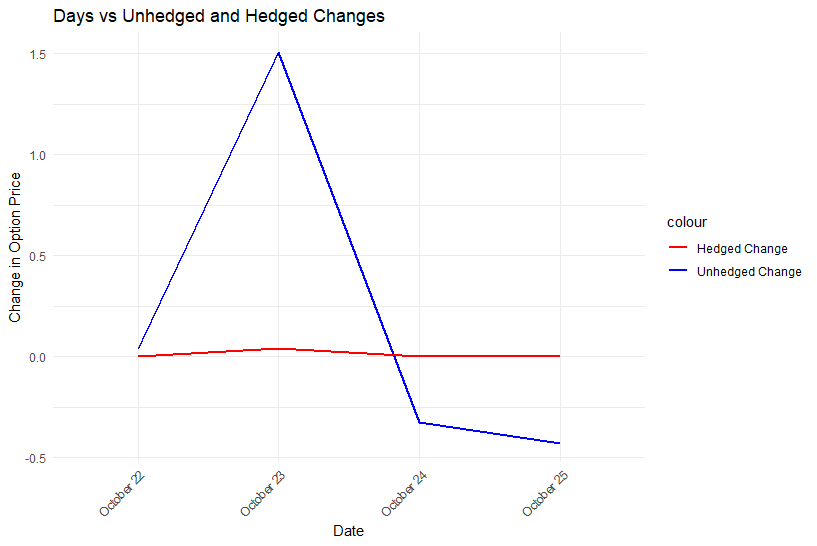
\includegraphics[width=0.65\linewidth]{content/images/hedgedvsunhedged.png}
    \caption{Comparison of change in Option Price of a hedged investment vs unhedged investment}
    \label{fig:hedgingvunhedging}
\end{figure}

\section{Gamma (\(\Gamma\))}

Gamma (\(\Gamma\)) for a barrier option measures the rate of change of delta (\(\Delta\)) with respect to changes in the underlying asset price (\(S\)). It represents the curvature or sensitivity of delta in response to movements in the underlying price. It provides insights into how rapidly an option's delta will change as the underlying price fluctuates.
\[
\Gamma = \frac{\partial^2 \text{Option Price}}{\partial S^2}
\]

For \textbf{knock-in} and \textbf{knock-out} barrier options, gamma exhibits unique behavior due to the presence of the barrier. The interaction between the price of the stock, the barrier level and the time to maturity influences how gamma behaves in different scenarios.

\begin{center}
	\begin{table}[H]
		\begin{tabular}{ | m{3cm} | m{5cm}| m{4cm} | m{4cm}|} 
			\hline
			\textbf{Barrier Type} & \textbf{Price Far from Barrier} & \textbf{Price Near the Barrier} & \textbf{Intuition}  \\ 
			\hline
			\textbf{Knock-Out} & Similar to vanilla options     & $\Gamma \uparrow$ as $S \to B$  & Gamma spikes as the price nears the barrier due to increased risk of knock-out. \\ 
			\hline
			\textbf{Knock-In}    & $\Gamma \approx 0$ far from barrier   & $\Gamma \uparrow$ as $S \to B$  & Gamma rises as the stock price approaches the barrier due to increased probability of activation. \\ 
			\hline
		\end{tabular}
		\caption{Gamma behavior for Knock-In and Knock-Out barrier options.}
		\label{tab:gamma_barrier_options}
	\end{table}
\end{center}

Figure~\ref{fig:gamma_behavior} illustrates the gamma behavior of an up-and-out put option as a function of the underlying stock price (\(S\)). As soon as the barrier is hit, the option is knocked out and gamma goes to zero. Gamma hedging is a risk management strategy used in options trading to mitigate the risks associated with large movements in the underlying asset's price. These large movements may cause large losses in delta hedged portfolio. Figure \ref{fig:compare_deltagamma_hedge} shows that hedging both delta and gamma provides minimum risk investment.

\begin{figure}[h]
    \centering
    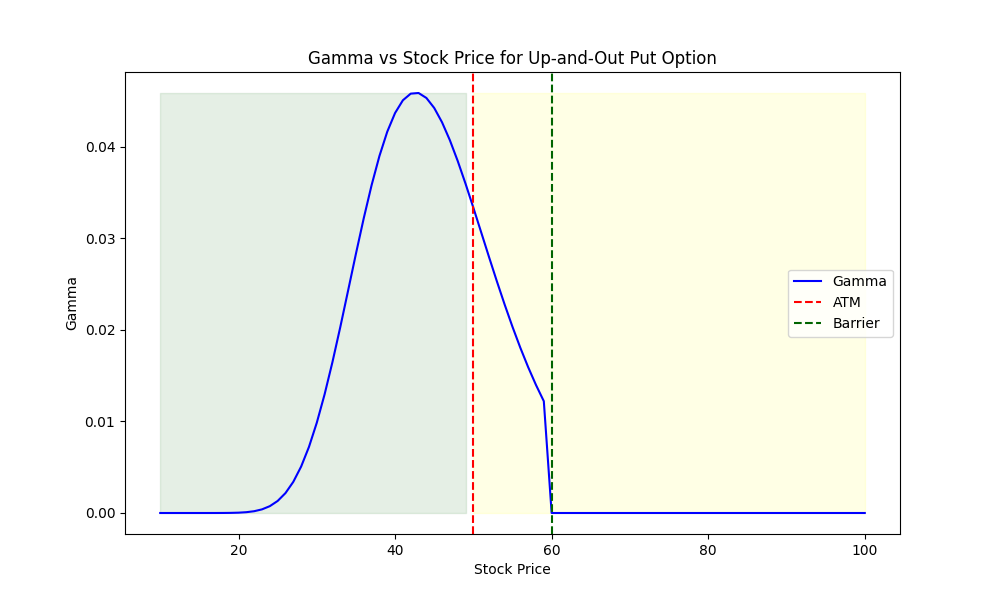
\includegraphics[width=.65\linewidth]{content/images/gamma.png}
    \caption{Gamma of an up-and-out put option vs. the Stock Price.}
    \label{fig:gamma_behavior}
\end{figure}

\begin{figure}[h]
    \centering
    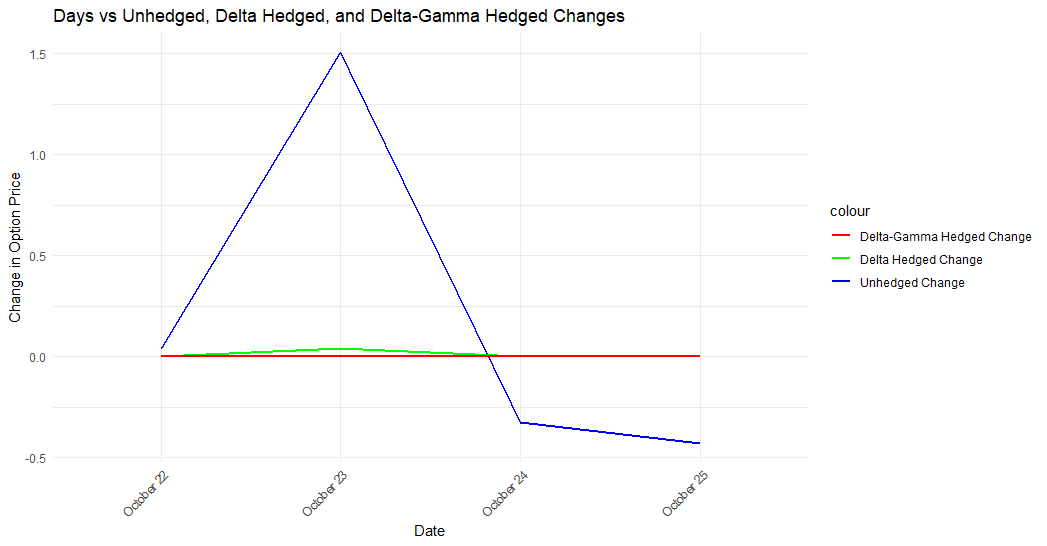
\includegraphics[width=.65\linewidth]{content/images/compare_hedging.png}
    \caption{Comparing different hedging results}
    \label{fig:compare_deltagamma_hedge}
\end{figure}


\begin{figure}[h]
    \centering
    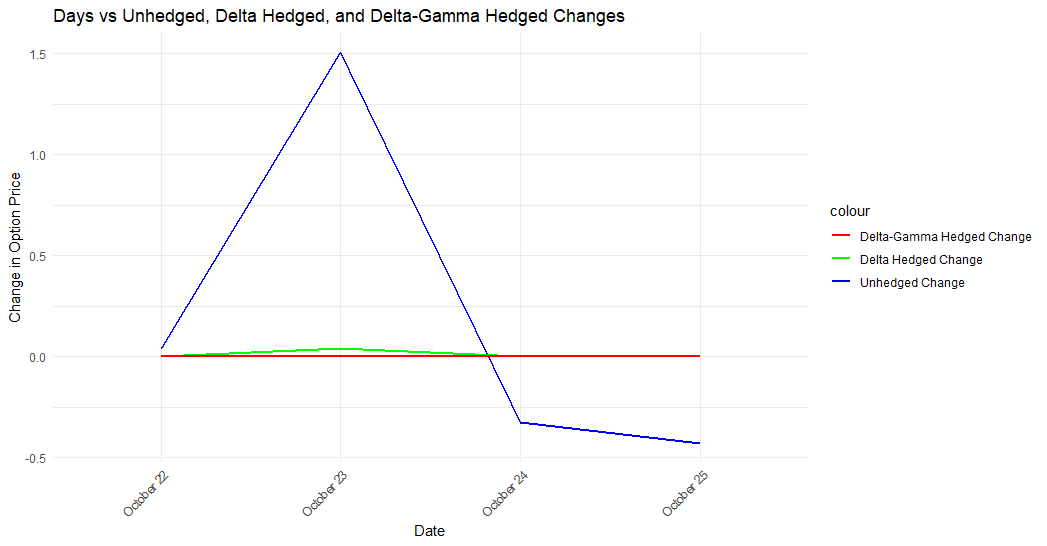
\includegraphics[width=.65\linewidth]{content/images/compare_hedging.png}
    \caption{Comparing different hedging results}
    \label{fig:compare_deltagamma_hedge}
\end{figure}


\begin{figure}[h]
	\centering
	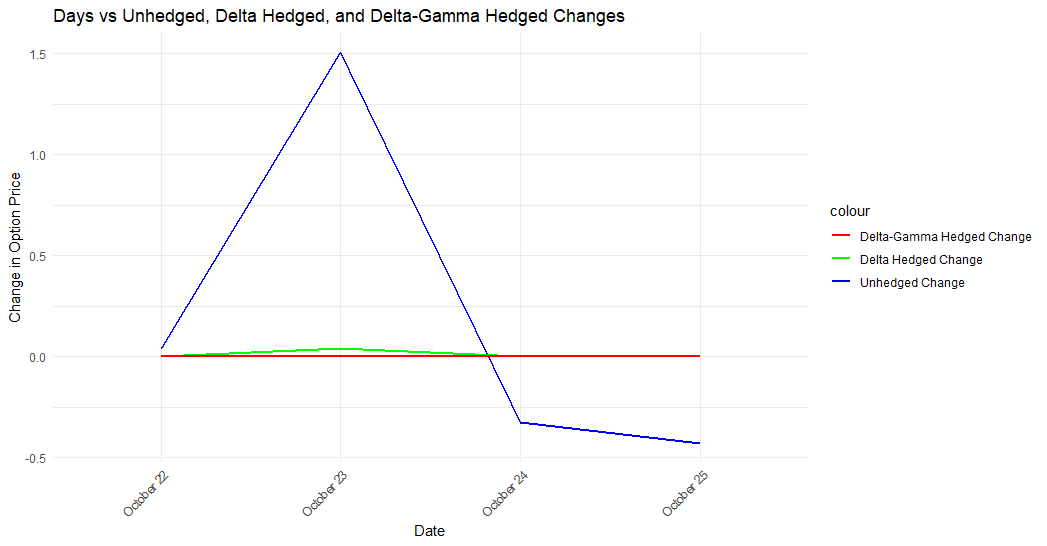
\includegraphics[width=.65\linewidth]{content/images/compare_hedging.png}
	\caption{Comparing different hedging results}
	\label{fig:compare_deltagamma_hedge}
\end{figure}


\section{Vega ($nu$)}

\textbf{Vega (\(\nu\))} measures the sensitivity of the option price to changes in volatility. For barrier options, the calculation of vega incorporates adjustments to account for the probability of breaching the barrier level under varying volatility conditions.
\[
\nu = \frac{\partial \text{Option Price}}{\partial \sigma}
\]

\begin{itemize}
	\item \textbf{Knock-In Options:} Increased volatility raises the likelihood of the underlying asset price crossing the barrier level, making the option more valuable. As a result, \(\nu\) (vega) will generally be positive.
	\item \textbf{Knock-Out Options:} Increased volatility can lead to a higher probability of the option being knocked out, reducing its value. Therefore, \(\nu\) will tend to be negative for these types of options.
\end{itemize}

\begin{figure}[H]
    \centering
    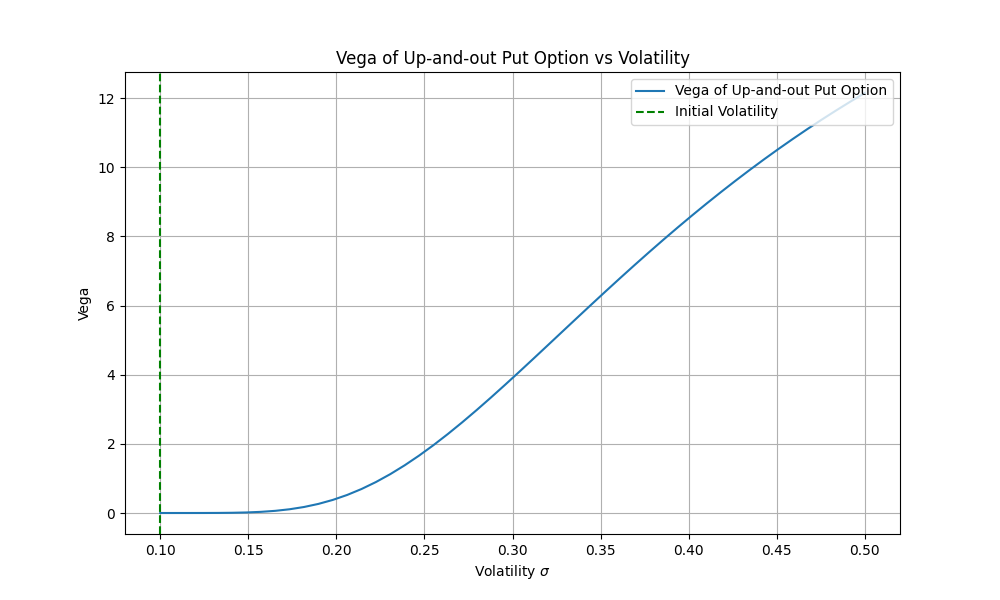
\includegraphics[width=.65\linewidth]{content/images/vega_upout.png}
    \caption{Vega vs Stock Price of an Up-and-Out Put Option}
    \label{fig:vega_behavior}
\end{figure}

The visualization shown in Figure~\ref{fig:vega_behavior} provides insights into how Vega behaves with changes in stock price across up-and-out put option. The sensitivity patterns are influenced by the interplay between volatility and the probability of breaching the barrier level. As the barrier is breached, vega immediately goes to zero.

\section{Theta ($Theta$)}

Theta (\(\Theta\)) measures the rate of change of an option's price with the passage of time, assuming all other variables remain constant. It is a critical "Greek" that reflects time decay, which is the gradual erosion of the option's value as expiration approaches. In the case of barrier options, theta is influenced not only by the time remaining but also by the interaction with the barrier level and the path dependency of the option.

Barrier options are unique because their payoff depends on the underlying asset price crossing (or not crossing) a specified barrier level during the option's lifetime. As such, the sensitivity of theta changes depending on proximity to the barrier, time remaining until maturity, and whether the option is near the knock-in or knock-out condition.

\begin{itemize}
    \item \textbf{Knock-In Options:} As time to maturity decreases, the value of knock-in options tends to decline, especially when the underlying asset price is far from the barrier. This is because the likelihood of triggering the option by crossing the barrier becomes lower as time runs out.
    
    \item \textbf{Knock-Out Options:} As time to maturity approaches, the risk of the underlying price reaching the barrier and knocking out the option increases, thereby accelerating time decay.
\end{itemize}


\begin{figure}[H]
    \centering
    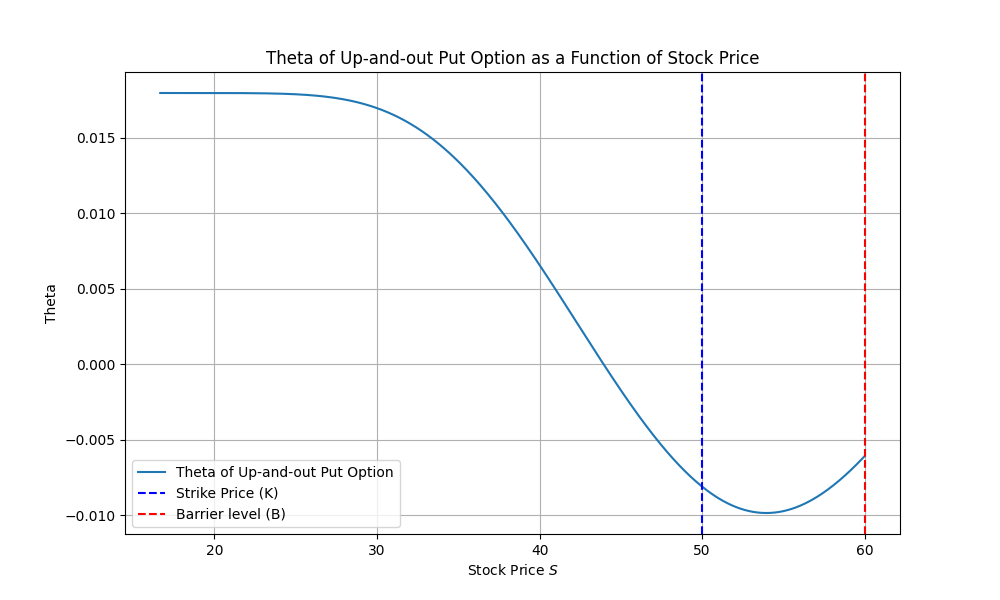
\includegraphics[width=.65\linewidth]{content/images/theta.png}
    \caption{Theta vs Stock Price of an Up-and-Out Put Option}
    \label{fig:theta_behavior}
\end{figure}


The visualization in Figure~\ref{fig:theta_behavior} illustrates the relationship between stock price and theta for an up-and-out put option. This analysis highlights how theta's sensitivity varies depending on proximity to the barrier. As the stock price approaches the strike, theta is decreasing. As the stock price approaches the barrier, it is increasing. However, when stock price hits the barrier, theta immediately goes to zero.


\section{Rho (\(\rho\))}

Rho for barrier options measures the sensitivity of the option price to changes in the risk-free interest rate (\(r\)). It represents how much the value of the option changes when the risk-free rate changes by 1\%. Rho is important in understanding the impact of monetary policy, such as changes in interest rates, on the value of barrier options.

\[
\rho = \frac{\partial \text{Option Price}}{\partial r}
\]

When interest rates rise:
\begin{itemize}
	\item \textbf{Knock-In Options:} Tend to show a positive relationship with Rho (\(\rho\)). This reflects that higher interest rates increase the present value of the potential payoff, making the knock-in option more valuable.
	\item \textbf{Knock-Out Options:} Tend to show muted sensitivity to changes in the interest rate. This is because the likelihood of being knocked out (and thus losing value) dominates any benefit gained from higher interest rates.
\end{itemize}
\begin{figure}[H]
    \centering
    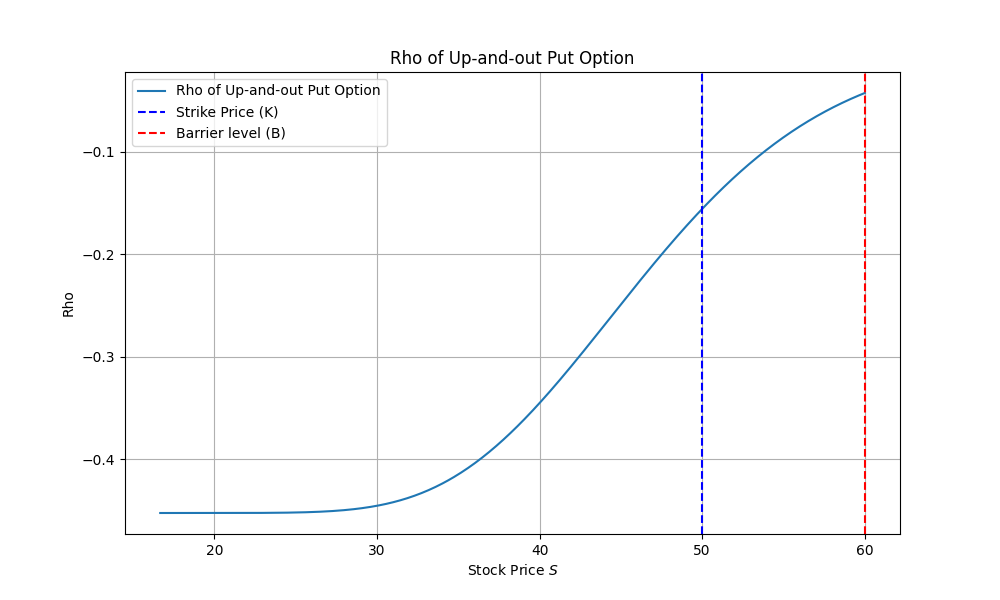
\includegraphics[width=.65\linewidth]{content/images/rho.png}
    \caption{Rho vs Stock Price for an Up-and-Out Put Option}
    \label{fig:rho_behavior}
\end{figure}

The visual behavior in Figure~\ref{fig:rho_behavior} illustrates how changes in the stock price (\(r\)) impact rho of an up-and-out barrier option. As the stock price increase, rho also increases. However, as stock price breaches the barrier, rho goes to zero.